\textbf{Block parameters for SRF-PLL simulink model}

\begin{figure}
    \centering
    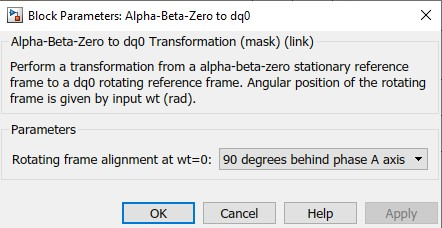
\includegraphics[width=0.5\textwidth]{ab0 to dq0.jpg}
    \caption{$\alpha \beta$ 0 to DQ0 block}
    \label{alpha beta 0 to DQ0 block}
\end{figure}

\begin{figure}
    \centering
    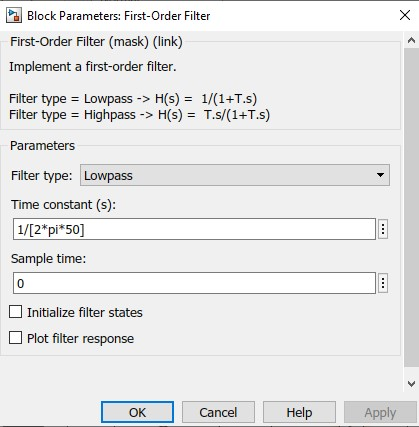
\includegraphics[width=0.5\textwidth]{low pass filter.jpg}
    \caption{low pass filter used in generation of alpha beta signals}
    \label{low pass filter}
\end{figure}



\begin{figure}
    \centering
    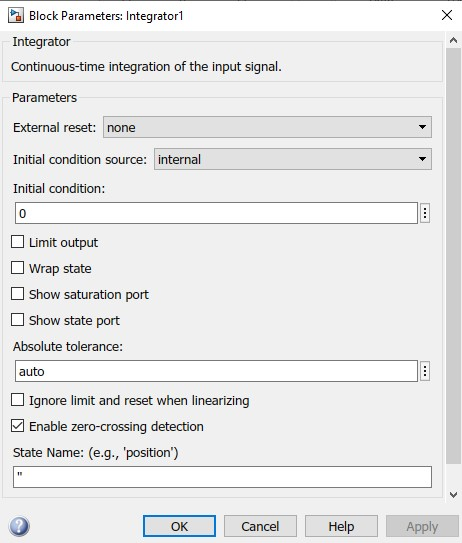
\includegraphics[width=0.5\textwidth]{intergrator.jpg}
    \caption{Integrator}
    \label{Integrator}
\end{figure}

\begin{figure}
    \centering
    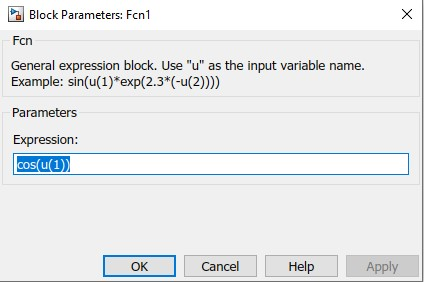
\includegraphics[width=0.5\textwidth]{fcn.jpg}
    \caption{fcn block ($\cos$)}
    \label{fcn block}
\end{figure}



\begin{figure}
    \centering
    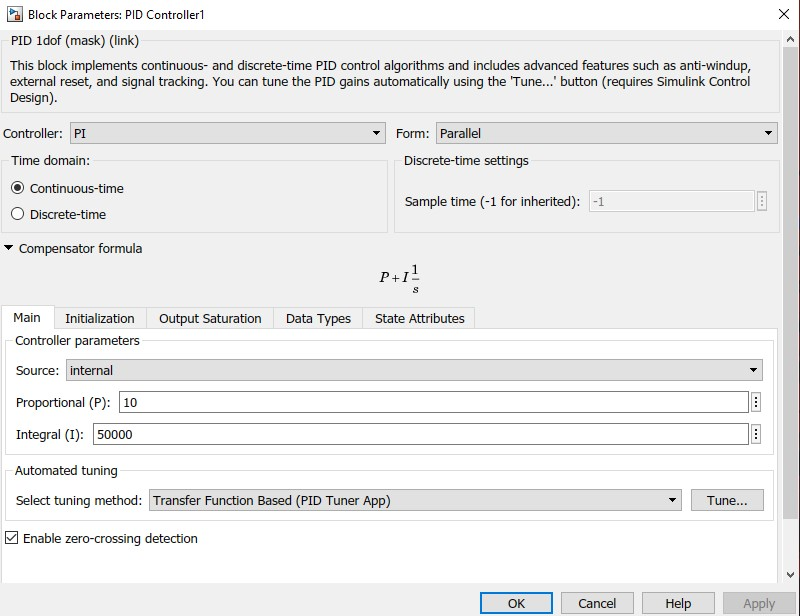
\includegraphics[width=1.0\textwidth]{PI controller.jpg}
    \caption{PI controller}
    \label{PI controller}
\end{figure}

\textbf{Code generation configurations}
\begin{figure}
    \centering
    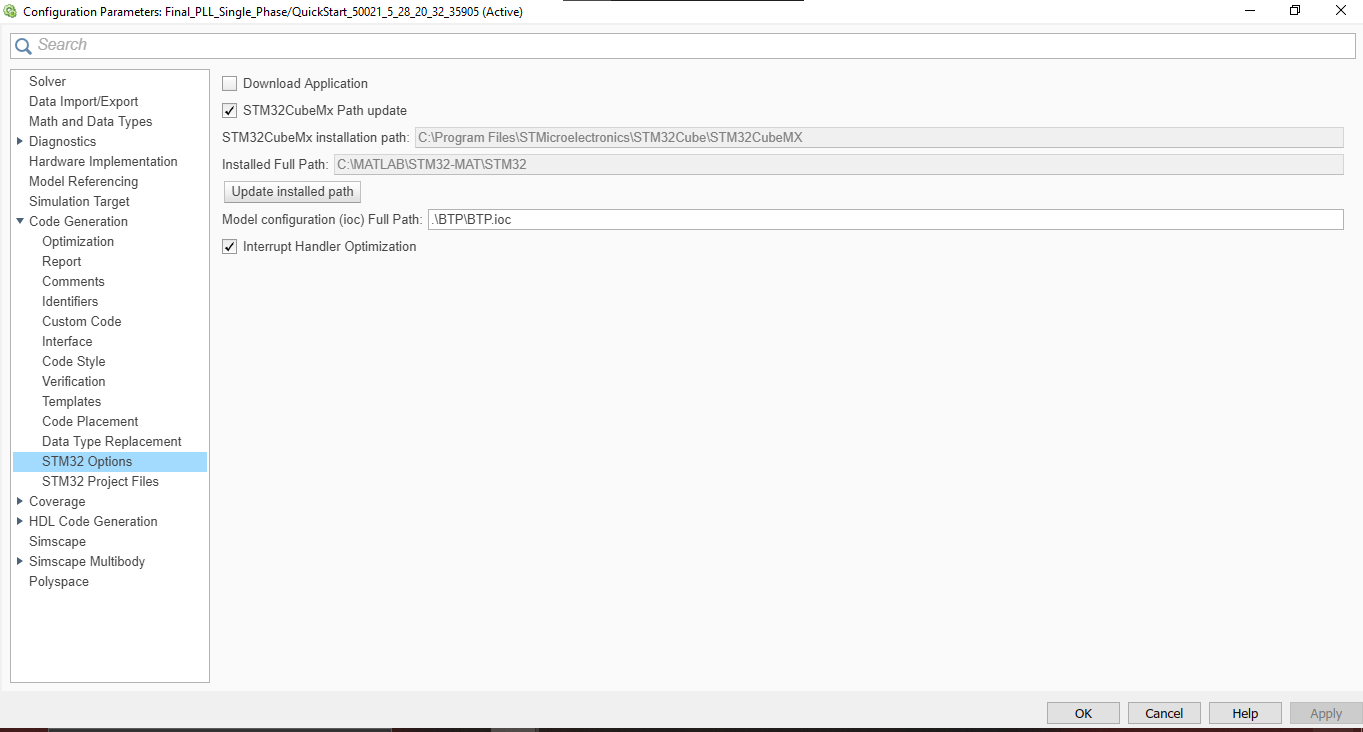
\includegraphics[width=1.0\textwidth]{Code generation_Solver.png}
    \caption{STM32CubeMX model configuration file}
    \label{Code generation_Solver.png}
\end{figure}

\begin{figure}
    \centering
    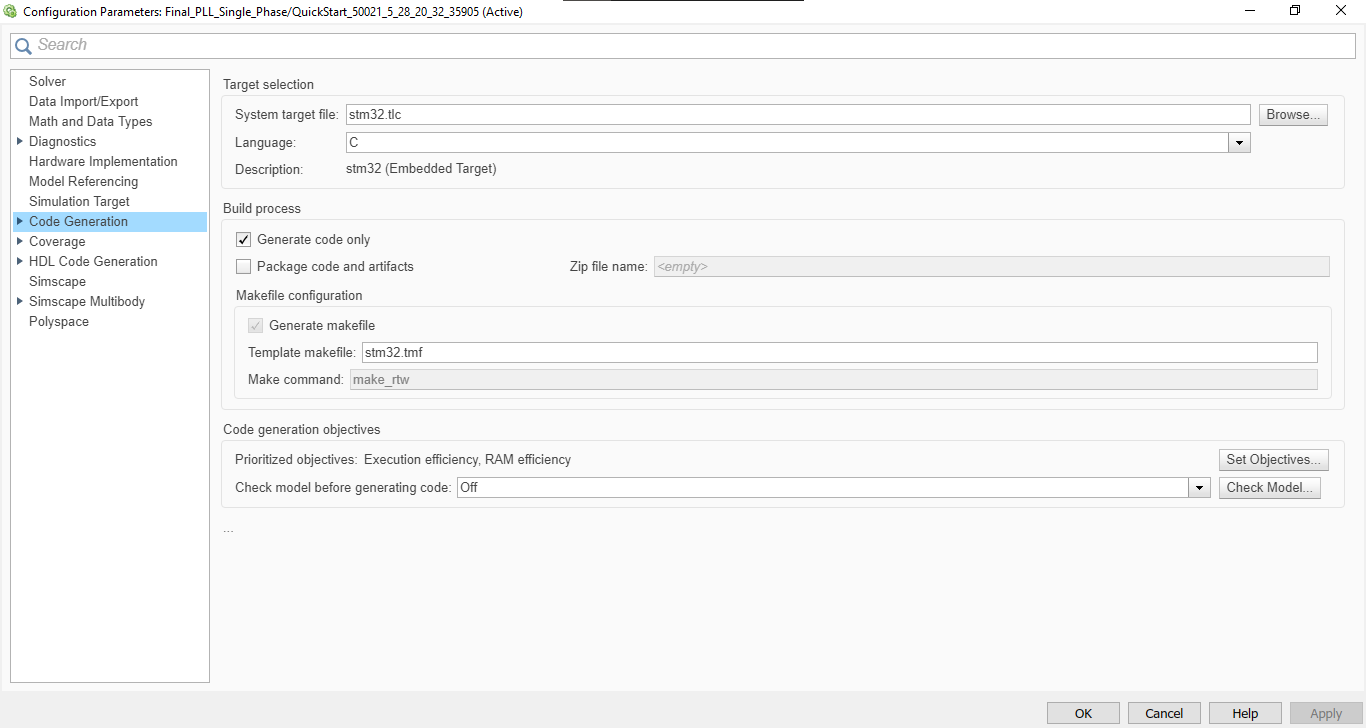
\includegraphics[width=1.0\textwidth]{Code generation.png}
    \caption{Code generation parameters}
    \label{Code generation.png}
\end{figure}